\documentclass{beamer}
\usepackage{mathtools}
\usepackage{graphicx}
\usepackage{tikz}

\graphicspath{{images/}}

\usetheme{Madrid}

\newcommand*{\ex}{\textnormal{ex}}

\title{Double Turán Problem}
\author{Ray Tsai}
\date{\today}

\begin{document}

\frame{\titlepage}

\begin{frame}{Overview}
  \tableofcontents
\end{frame}

\section{Introduction}

\begin{frame}
\frametitle{Introduction}
What is the Turán problem? \pause

\begin{block}{Question}
  Given a graph $F$, how many edges can an $n$-vertex graph have while containing no copy of $F$ as a subgraph?
\end{block}
\end{frame}

\begin{frame}
\frametitle{Introduction}

Let $F$ be a graph. We call the following quantity the \textit{Turán number} or \textit{extremal number} of $F$:

\begin{block}{Definition}
  \[
    \ex(n, F) \coloneq \max \{ e(G) : |V(G)| = n \text{ and } F \not\subseteq G \}
  \]
\end{block}
\end{frame}
\begin{frame}
  \frametitle{Introduction}

  \begin{block}{Turán's theorem}
    The maximum number of edges in an $n$-vertex graph containing no clique of order $r + 1$ is $e(T_r(n))$, with equality only for $T_r(n)$.
  \end{block}
\end{frame}

\begin{frame}
  \frametitle{Introduction}

  \begin{block}{Erd\H{o}s-Stone Theorem, Simonovits' Theorem}
    Let $F$ be any graph of chromatic number $r + 1 \geq 3$. Then $\ex(n, F) = (1 + o(1))T_r(n)$ as $n \rightarrow \infty$.
  \end{block}
\end{frame}

\begin{frame}
\frametitle{Double Turán Problem}

What is the double Turán problem? \pause

\vspace{0.5cm}

Let $G_1, G_2, \ldots, G_m$ be graphs on $[n]$ with $E(F) \not\subseteq E(G_i) \cap E(G_j)$ for distinct $i, j \in [m]$. \pause (\textit{Double $F$-free})

\pause

\begin{block}{Question}
  What is the value of $\phi(m, n, F) = \max \sum_{i = 1}^m G_i$?
\end{block}
\end{frame}

\section{Double Turán Problem}

\begin{frame}
  \frametitle{Double Turán Problem}

  Double Turán problems are closely related to Turán problems for $3$-uniform hypergraphs $H$ through \textit{link graphs}.

  \pause

  \vspace{0.3cm}

  \begin{block}{Definition}
    For $i \in V(H)$, define graph $H_i$ with
    \[
      V(H_i) = V(H) \backslash \{i\} \quad \text{and} \quad E(H_i) = \{\{j, k\} : \{i, j, k\} \in E(H)\}.
    \]
  \end{block}
\end{frame}

\begin{frame}
  \frametitle{Double Turán Problem}

  Example: Octahedron-free 3-uniform hypergraph $H$

  \pause

  \begin{figure}
    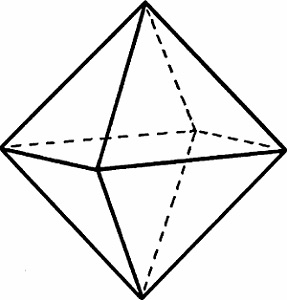
\includegraphics[width=0.15\linewidth]{oct}
    \caption{Octahedron $O$}
    \centering
  \end{figure}

  \pause

  \begin{center}
    $H$ is octahedron-free $\implies$ $H_1, H_2, \ldots, H_n$ are double $C_4$-free.
  \end{center}

  \pause

  \[
    \boxed{\ex(n, O) \leq \phi(n, n, C_4)}
  \]
\end{frame}

\section{Induced Double Turán Problem}

\begin{frame}
  \frametitle{Induced Double Turán Problem}

  What is the \textit{induced} double Turán problem? \pause

  \begin{block}{Definition}
    We call graphs $G_1, G_2, \ldots, G_m$ \textit{induced} if each $G_i$ is an induced subgraph of $\bigcup_{i = 1}^m G_i$.
  \end{block}

  \pause

  \vspace{0.5cm}

  Let graphs $G_1, G_2, \ldots, G_m$ be induced and double $F$-free.

  \begin{block}{Question}
    What is the value of $\phi^*(m, n, F) = \max \sum_{i = 1}^m e(G_i)$?
  \end{block}
\end{frame}

\begin{frame}
  \frametitle{Induced Double Turán Problem}

  \begin{block}{Generalizaed Turán problem}
    What is the maximum number $\ex(n, F, K_3)$ of triangles in a graph $H$ on $[n]$ with no copy of $F$ as a subgraph?
  \end{block}

  \pause 

  \vspace{0.5cm}

  For $i \in V(G)$, define $G_i$ with
  \[
    V(G_i) = V(G) \quad \text{and} \quad E(G_i) = \{\{j, k\} : \{i, j\}, \{j, k\}, \{i, k\} \in E(G)\}
  \]
\end{frame}

\begin{frame}
  \frametitle{Induced Double Turán Problem}

  Ex. Octahedron-free graph $G$.

  \begin{figure}
    \begin{minipage}{0.48\textwidth}
      \centering
      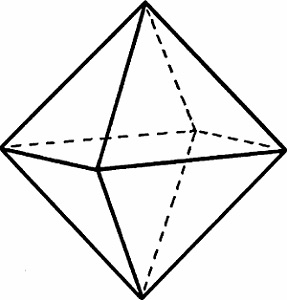
\includegraphics[width=0.45\linewidth]{oct}
      \caption{Octahedron}
    \end{minipage}
    \hfill
    \begin{minipage}{0.48\textwidth}
      \centering
      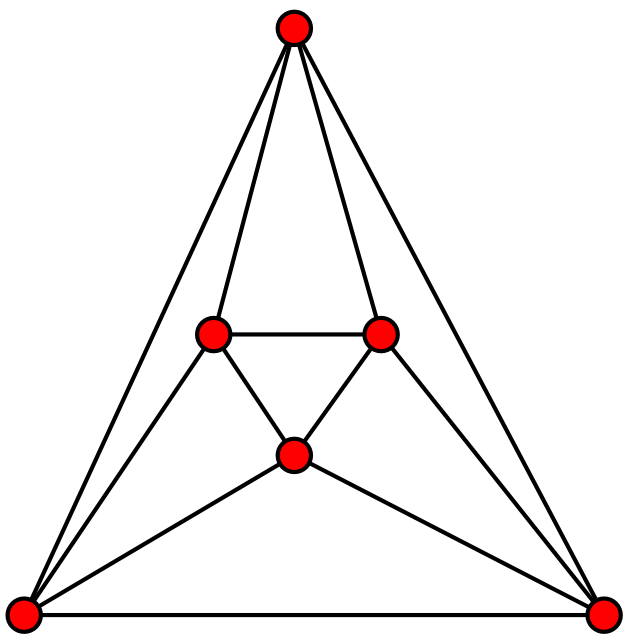
\includegraphics[width=0.45\linewidth]{Octahedron_graph}
      \caption{Octahedron Graph $K_{2,2,2}$}
    \end{minipage}
  \end{figure}

  \pause

  \vspace{0.1cm}

  \begin{center}
    $G$ is $K_{2,2,2}$-free $\implies$ $G_1, G_2, \ldots, G_n$ are double $K_{2, 2}$-free.
  \end{center}

  \pause

  \[
    \boxed{\ex(n, K_{2,2,2}, K_3) \leq \phi(n, n, K_{2,2})}
  \]
\end{frame}

\section{Main Results}

\begin{frame}
  \frametitle{Main Results}


  \begin{block}{Theorem A}
    For $m \geq 3$ and non-bipartite $F$, if $n$ is large enough, then
    \[
      \phi^*(m, n, F) = m \cdot \ex(n, F),
    \]
    with equality only for identical extremal $n$-vertex $F$-free graphs.
  \end{block}

  \pause

  \begin{block}{Theorem B}
    For $m, n, r \geq 3$,
    \[
      \phi^*(m,n,K_{r}) = m \cdot e(T_{r - 1}(n)),
    \]
    with equality for induced $K_{r}$-free graphs $G_1, G_2, \dots, G_m$ only if $G_1 = G_2 = \dots = G_m = T_{r - 1}(n)$.  
  \end{block}
\end{frame}

\begin{frame}
  \frametitle{Main Results}

  We need the idea of \textit{$(m, n, k)$-blowup} to state the result for $\phi(m, n, K_r)$.

  \pause

  \begin{figure}
    \centering
    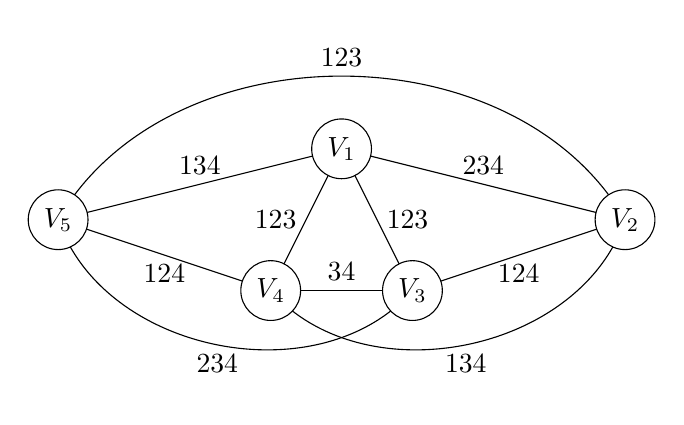
\begin{tikzpicture}[scale=0.9]
    \draw[bend right=60] (4, 0.5) to node[midway, above] {$123$} (-4, 0.5); 
    \draw (-4, 0.5) to node[midway, below] {$124$} (-1, -0.5); 
    \draw (-1, -0.5) to node[midway, above] {$34$} (1, -0.5); 
    \draw (1, -0.5) to node[midway, below] {$124$} (4, 0.5); 
    \draw (0, 1.5) to node[midway, above] {$234$} (4, 0.5); 
    \draw (0, 1.5) to node[midway, above] {$134$} (-4, 0.5); 
    \draw (0, 1.5) to node[midway, left] {$123$} (-1, -0.5); 
    \draw (0, 1.5) to node[midway, right] {$123$} (1, -0.5); 
    \draw[bend left=60] (4, 0.5) to node[midway, below] {$134$} (-1, -0.5); 
    \draw[bend right=60] (-4, 0.5) to node[midway, below] {$234$} (1, -0.5);

    \foreach [count=\i] \x/\y in {0/1.5, 4/0.5, 1/-0.5, -1/-0.5, -4/0.5} { 
      \fill[white] (\x, \y) circle (12pt);
      \draw (\x, \y) circle (12pt);
      \node at (\x, \y) [] {$V_{\i}$}; 
    }
    \end{tikzpicture}
    \caption{Example of an $(4, n, 5)$-blowup not containing a double $K_3$.}
  \end{figure}
\end{frame}

\begin{frame}

  \frametitle{Main Results}

  Let $f(m, n, r)$ denote the maximum possible sum of edges in an double $K_r$-free $(m, n, k)$-blowup with $k \leq \binom{m}{2}$.

  \pause

  \begin{block}{Theorem C}
    For $n \geq 1$,
    \begin{enumerate}
      \item 
      \[
        \phi(3, n, K_3) = \binom{n}{2} + \left\lfloor \frac{n^2}{2} \right\rfloor.
      \]
      \item if $r \geq 2$ and $m \geq 1$,
      \[
        \phi(m, n, K_r) = f(m, n, r).
      \]
    \end{enumerate}
    In particular,
    \[
      \lim_{n \to \infty} \frac{f(4, n, 3)}{\binom{n}{2} + \left\lfloor \frac{n^2}{2} \right\rfloor} > 1
    \]
  \end{block}
\end{frame}

\begin{frame}
  \frametitle{Main Results}

  \begin{block}{Conjecture}
    Let $F$ be any non-empty graph and $m, n \geq 1$. Then
    \[ 
      \phi^*(m,n,F) = \Theta(m \cdot \ex(n,F) + n^2).
    \]
  \end{block}

  \pause

  \vspace{0.3cm}

  \[ 
    \phi^*(m,n,F) \geq \max\Bigl\{\binom{n}{2},m\cdot \ex(n,F)\Bigr\}.
  \]
\end{frame}

\begin{frame}
  \frametitle{Main Results}

  \begin{block}{Conjecture}
    Let $F$ be any non-empty graph and $m, n \geq 1$. Then
    \[ 
      \phi^*(m,n,F) = \Theta(m \cdot \ex(n,F) + n^2).
    \]
  \end{block}

  \vspace{0.5cm}

  By Theorem 1, the conjecture is true when $F$ is non-bipartite.
\end{frame}

\begin{frame}
  \frametitle{Main Results}

  \begin{block}{Conjecture}
    Let $F$ be any non-empty graph and $m, n \geq 1$. Then
    \[ 
      \phi^*(m,n,F) = \Theta(m \cdot \ex(n,F) + n^2).
    \]
  \end{block}

  \vspace{0.3cm}

  Since
  \[
    \ex(n, K_{2, 2, 2}, K_3) \leq \phi^*(n, n, K_{2, 2})
  \]
  the conjecture implies
  \[
    \ex(n, K_{2, 2, 2}, K_3) \leq O(n^{2})
  \]
\end{frame}

\begin{frame}
  \frametitle{Main Results}

  \begin{block}{Theorem D}
    Let $F$ be a graph. If there exists an extremal $F$-free $n$-vertex graph with maximum degree at most $\sqrt{n}/m^2$, then 
    \[ 
      \phi(m, n, F) = \binom{n}{2} + \binom{m}{2}\ex(n,F).
    \]
  \end{block}

  \pause

  \vspace{0.3cm}

  If $P$ is a path of length $2$ and $m = o(n^{1/4})$, 
  \[
    \binom{n}{2} + m - 1 \leq \phi^*(m, n, P) \leq \phi(m, n, P) = \binom{n}{2} + \binom{m}{2} \left\lfloor \frac{n}{2}\right\rfloor. 
  \]
\end{frame}

\begin{frame}
  \frametitle{Main Results}

  \begin{block}{Theorem E}
    Let $P$ be a path with two edges. Then $\phi(n, n, P) = \Omega(n^{5/2})$, whereas $\phi^*(n, n, P) = o(n^{5/2})$, as $n \rightarrow \infty$. In particular, 
    \[ 
      \lim_{n \rightarrow \infty} \frac{\phi^*(n, n, P)}{\phi(n, n, P)} = 0.
    \]
  \end{block}

  \pause

  \vspace{0.3cm}

  This shows that $\phi(n, n, P)$ and $\phi^*(n, n, P)$ are very different problems.
\end{frame}

\section{Proof of Theorem B}

\begin{frame}
  \frametitle{Proof of Theorem B}

  \begin{block}{Theorem B}
    Let $m, n, r \geq 3$. Then 
    \[
      \phi^*(m,n,K_{r}) = m \cdot e(T_{r - 1}(n)),
    \]
    with equality for induced $K_{r}$-free graphs $G_1, G_2, \dots, G_m$ only if $G_1 = G_2 = \dots = G_m = T_{r - 1}(n)$.  
  \end{block}

  \vspace{0.3cm}

  Proof Roadmap

  \begin{itemize}
    \item Step 1: Reduce to the case of smaller $m$
    \item Step 2: Further reduce to an optimization problem
    \item Step 3: Solve the optimization problem
  \end{itemize}
\end{frame}

\begin{frame}
  \frametitle{Step 1: Reduce to the case of smaller $m$}

  Proof Roadmap

  \begin{itemize}
    \item \textbf{Step 1:} Reduce to the case of smaller $m$
    \item \textcolor{gray}{Step 2: Further reduce to an optimization problem}
    \item \textcolor{gray}{Step 3: Solve the optimization problem}
  \end{itemize}
\end{frame}

% \begin{frame}
%   \frametitle{Step 1: Reduce to the case of smaller $m$}

%   Let $G_1, \ldots, G_m$ be induced double $F$-free graphs on $[n]$.

%   \begin{block}{Lemma 1}
%     For $2 \leq k \leq m$,
%     \[
%       \phi^*(m,n,F) \leq \frac{m}{k} \cdot \phi^*(k, n, F).
%     \]
%     Moreover, suppose $\sum_{i = 1}^k e(G_i) = \phi^*(k, n, F)$ only if $G_1 = \cdots = G_k$. Then $\sum_{i = 1}^m e(G_i) = \phi^*(m, n, F)$ only if $G_1 = \cdots = G_m$.
%   \end{block}
% \end{frame}

% \begin{frame}
%   \frametitle{Step 1: Reduce to the case of smaller $m$}

%   Put $G_{i + m} = G_i$ for all $i \in [m]$.
%   \[
%     \sum_{i = 1}^m e(G_i) 
%     = \frac{1}{k}\sum_{i = 1}^m [e(G_i) + \cdots + e(G_{i + k - 1})]
%   \]

%   \pause

%   Since $e(G_i) + \cdots + e(G_{i + k - 1}) \leq \phi^*(k, n, F)$,
%   \[
%     \sum_{i = 1}^m e(G_i) \leq \frac{m}{k} \cdot \phi^*(k, n, F).
%   \]
% \end{frame}

% \begin{frame}
%   \frametitle{Step 1: Reduce to the case of smaller $m$}

%   Suppose $\sum_{i = 1}^m e(G_i) = \frac{m}{k} \cdot \phi^*(k, n, F)$ and $G_1 \neq G_2$. 

%   \pause

%   \vspace{0.5cm}

%   By assumption $\sum_{i = 1}^k e(G_i) < \phi^*(k, n, F)$. 

%   \pause

%   \vspace{0.5cm}
  
%   $\implies e(G_i) + \cdots + e(G_{i + k - 1}) > \phi^*(k, n, F)$ for some $i > 1$.

%   \vspace{0.5cm}

%   $\sum_{i = 1}^k e(G_i) = \phi^*(k, n, F)$ only if $G_1 = \cdots = G_k \implies \sum_{i = 1}^m e(G_i) = \phi^*(m, n, F)$ only if $G_1 = \cdots = G_m$.
% \end{frame}

\begin{frame}
  \frametitle{Step 2: Further reduce to an optimization problem}

  Proof Roadmap

  \begin{itemize}
    \item Step 1: Reduce to the case of smaller $m$
    \item \textbf{Step 2:} Further reduce to an optimization problem
    \item \textcolor{gray}{Step 3: Solve the optimization problem}
  \end{itemize}
\end{frame}

\begin{frame}
  \frametitle{Step 2: Further reduce to an optimization problem}

  \begin{center}
    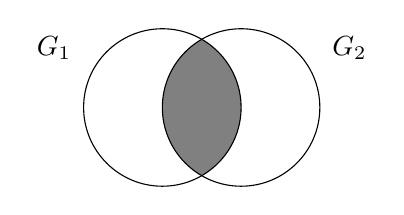
\begin{tikzpicture}
      % ---- fill only the intersection -----------------
      \begin{scope}
        \clip (0,0) circle (1);          % keep area inside left circle
        \fill[gray] (1,0) circle (1);    % paint overlap with right circle
      \end{scope}
    
      % ---- circle outlines ----------------------------
      \draw (0,0) circle (1);
      \draw (1,0) circle (1);
    
      % ---- labels outside the circles -----------------
      \node[left=1pt]  at (-1,0.75) {$G_1$};
      \node[right=1pt] at (2,0.75) {$G_2$};
    \end{tikzpicture}
  \end{center}

  \pause

  \begin{block}{Observation}
    If $G_1, G_2$ intersects in $t$ vertices, Then
    \[
      e(G_1) + e(G_2) \leq \binom{n - t}{2} + (n - t)t + 2\ex(t, F)
    \]
  \end{block}

  \pause

  \vspace{0.3cm}

  $\implies$ we are done if the unique maximum is at $t = n$.
\end{frame}

\begin{frame}
  \frametitle{Step 3: Solve the optimization problem}

  Proof Roadmap

  \begin{itemize}
    \item Step 1: Reduce to the case of smaller $m$
    \item Step 2: Further reduce to an optimization problem
    \item \textbf{Step 3:} Solve the optimization problem
  \end{itemize}
\end{frame}

% \begin{frame}
%   \frametitle{Step 3: Solve the optimization problem}

%   By Lemma 1, it suffices prove the case $m = 3$. 

%   \pause

%   \vspace{0.6cm}

%   Let $G_1, G_2, G_3$ be induced double $K_r$-free graphs, such that $e(G_1) + e(G_2) + e(G_3) = \phi^*(3, n, K_r)$ and $e(G_1) \geq e(G_2) \geq e(G_3)$.

%   \pause

%   \vspace{0.6cm}

%   Since $\phi^*(3, n, K_r) \geq 3\ex(n, K_r)$, we must have $e(G_1) + e(G_2) \geq 2\ex(n, K_r)$.

%   \pause

%   \vspace{0.6cm}

%   Since $G_1, G_2, G_3$ are induced, we only need to show $G_1 = G_2 = T_{r - 1}(n)$.
% \end{frame}

% \begin{frame}
%   \frametitle{Step 3: Solve the optimization problem}

%   Let $t = |V(G_1 \cap G_2)|$. By Turán's Theorem,
%   \[
%     \ex(t, K_{r}) - \ex(t - 1, K_{r}) = t - \left\lceil \frac{t}{r - 1} \right\rceil.
%   \]

%   \pause

%   \vspace{0.5cm}

%   It follows that
%   \begin{align}
%     f(n, t, K_r) - f(n, t - 1, K_r)
%     &= - t + 1 + 2[\ex(t, K_r) - \ex(t - 1, K_r)] \notag \\
%     &= t + 1 - 2\left\lceil \frac{t}{r - 1} \right\rceil. 
%   \end{align}
% \end{frame}

% \begin{frame}
%   \frametitle{Step 3: Solve the optimization problem}

%   For $r \geq 4$,
%   \[
%     f(n, t, K_r) - f(n, t - 1, K_r) = t + 1 - 2\left\lceil \frac{t}{r - 1} \right\rceil > 0
%   \]

%   \pause

%   \vspace{0.5cm}

%   $\implies f(n, t, K_r)$ is strictly increasing on $t$.

%   \pause

%   \vspace{0.5cm}

%   $\implies t = n$ so that $e(G_1) + e(G_2) \geq 2\ex(n, F)$.

%   \pause

%   \vspace{0.5cm}

%   $\implies \phi^*(2, n, K_r) = 2\ex(n, F)$ and $G_1 = G_2 = T_{r - 1}(n)$.

%   \vspace{0.5cm}

%   This solves the case $r \geq 4$.
% \end{frame}

% \begin{frame}
%   \frametitle{Step 3: Solve the optimization problem}

%   For $r = 3$,
%   \[
%     f(n, t, K_r) - f(n, t - 1, K_r) = t + 1 - 2\left\lceil \frac{t}{2} \right\rceil \geq 0
%   \]

%   \pause

%   \vspace{0.5cm}

%   $\implies f(n, t, K_3)$ is non-decreasing on $t$ and $f(n, t, K_3) > f(n, t, K_3)$ for even $t$.

%   \pause

%   \vspace{0.5cm}

%   $\implies t = n$ or $t = n - 1$ so that $e(G_1) + e(G_2) \geq 2\ex(n, F)$.

%   \pause

%   \vspace{0.5cm}

%   $\implies \phi^*(2, n, K_3) = 2\ex(n, K_3)$, and either $G_1 = G_2 = T_{2}(n)$ or $G_2 = T_{2}(n - 1)$ and $G_1 = G_2 + K_1$.
% \end{frame}

% \begin{frame}
%   \frametitle{Step 3: Solve the optimization problem}

%   If $G_1 = G_2 = T_{2}(n)$ then we are done.

%   \pause

%   \vspace{0.5cm}

%   Suppose $G_2 = T_{2}(n - 1)$ and $G_1 = G_2 + K_1$. 

%   \pause

%   \vspace{0.5cm}

%   Since $e(G_1) + e(G_2) + e(G_3) \geq 3\ex(n, K_3)$,
%   \[
%     e(G_3) = \ex(n, K_3) > T_{2}(n - 1) = e(G_2),
%   \]
%   contradiction.

%   \pause

%   \vspace{0.5cm}

%   This solves Theorem B.
% \end{frame}

% \begin{frame}
%   \frametitle{Extra Ingredients to Prove Theorem A}

%   \begin{block}{Theorem A}
%     For $m \geq 3$ and non-bipartite $F$, if $n$ is large enough, then
%     \[
%       \phi^*(m, n, F) = m \cdot \ex(n, F),
%     \]
%     with equality only for identical extremal $n$-vertex $F$-free graphs.
%   \end{block}

%   \vspace{0.3cm}

%   \begin{itemize}
%     \item First show that $t = |V(G_1 \cap G_2)| \geq \sqrt{n}$.
%     \item For large enough $t$, any extremal $t$-vertex $F$-free graph contains a spanning $T_{r - 1}(t)$.
%   \end{itemize}
% \end{frame}

\section{Proof of Theorem C}

\begin{frame}
  \frametitle{Proof of Theorem C: Upper Bound}

  We need to show
  \[  
    \phi(m, n ,F) \leq \binom{n}{2} + \ex(n, F)\binom{m}{2}.  
  \]

  \pause
  
  Let $E_S$ be the set of edges in exactly $\{G_i\}_{i \in S}$.

  \pause

  \[
    \implies \sum_{i = 1}^m e(G_i) = \sum_{S \subseteq [m]} |S||E_S| \leq \binom{n}{2} + \sum_{S \subseteq [m], |S| \geq 2} (|S| - 1)|E_S|.
  \]
\end{frame}

\begin{frame}

  \frametitle{Proof of Theorem C: Upper Bound}

  \[
    \sum_{\substack{S \subseteq [m] \\ |S| \geq 2}} (|S| - 1)|E_S| = \sum_{\substack{S \subseteq [m], \\ |S| = 2}} \sum_{T \supseteq S} \frac{(|T| - 1)|E_T|}{\binom{|T|}{2}} \leq \sum_{\substack{S \subseteq [m], \\ |S| = 2}} \sum_{T \supseteq S} |E_T|,
  \]
  as each $T \in [m]$ with $|T| \geq 2$ is counted $\binom{|T|}{2}$ times.
\end{frame}

\begin{frame}
  \frametitle{Proof of Theorem C: Upper Bound}

  Observation: If $|S| \geq 2$, the edge set $\bigcup_{T \supseteq S} E_T$ is $F$-free.

  \pause

  \vspace{0.3cm}

  \[
    \left|\bigcup_{T \supseteq S} E_T\right| = \sum_{T \supseteq S} |E_T| \leq \ex(n, F)
  \]
  \pause

  \vspace{0.3cm}

  \[
    \implies \sum_{\substack{S \subseteq [m] \\ |S| \geq 2}} (|S| - 1)|E_S| \leq \sum_{\substack{S \subseteq [m], \\ |S| = 2}} \sum_{T \supseteq S} |E_T| \leq \binom{m}{2}\ex(n, F)
  \]
\end{frame}

\begin{frame}
  \frametitle{Proof of Theorem C: Lower Bound}

  Let $H_1, \ldots, H_{\binom{m}{2}}$ be extremal $F$-free graphs on $[n]$ with $\Delta(H_i) \leq \sqrt{n}/m^2$

  \pause

  \vspace{0.7cm}

  n.t.s. we can embed each $H_i$ onto $[n]$ s.t. edges are pairwise disjoint.

  \pause

  \vspace{0.7cm}

  IDEA: start with any embedding and iteratively decrease overlapping edges
\end{frame}

\begin{frame}
  \frametitle{Proof of Theorem C: Lower Bound}

  Define a \textit{$(u, v, i)$-swap} by swapping the embedding of vertex $u$ and $v$ of $H_i$

  \pause

  \vspace{0.7cm} 
  
  $\implies (u, v, i)$-swap perserves graph isomorphism.
\end{frame}

\begin{frame}
  \frametitle{Proof of Theorem C: Lower Bound}

  For vertex $v$, let $N(v) = N_{H_1}(v) \cup \cdots \cup N_{H_{\binom{m}{2}}}(v)$

  \pause

  \vspace{0.5cm} 

  Suppose there exists $\{u, w\} \in E(H_i) \cap E(H_j)$

  \pause

  \vspace{0.5cm} 

  $|N(u)| \leq M \cdot \triangle \leq n^{1/2}/2$

  \pause

  \vspace{0.5cm} 

  $\implies |N(u) \cup N(N(u))| \leq \triangle + \triangle(\triangle - 1) \leq n/4$

  \pause

  \vspace{0.5cm} 

  $\implies \exists v \notin N(u) \cup N(N(u))$, so $N(u) \cap N(v) = \emptyset$.

  \pause

  \vspace{0.5cm} 

  $\implies (u, v, i)$-swap makes $\{u, w\}$ not overlapping!

  \pause

  \vspace{0.5cm} 

  Keep swapping until no overlapping edges left

\end{frame}

\end{document}
